\chapter{3D CNN approach}
\section{Introduction}
\begin{figure}[h]
    \centering
    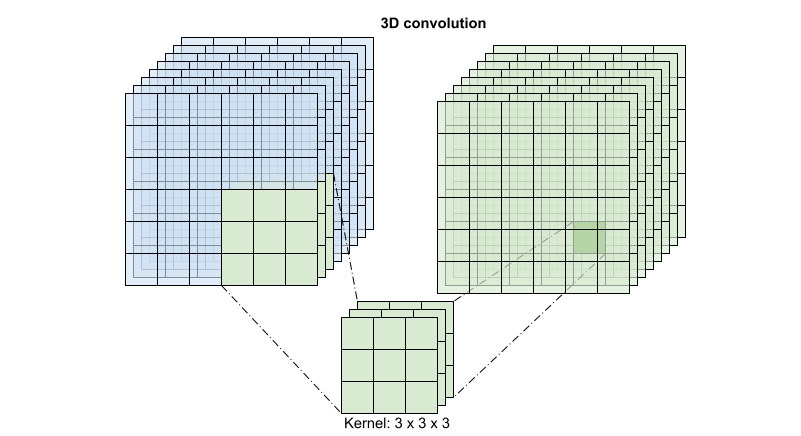
\includegraphics[width=\textwidth]{./images/3DCNN.png}
    \caption{How a 3D CNN works}
    \label{fig:How3DCNNWorks}
\end{figure}

2D CNN networks operate by applying convolutions spatially, traversing both the horizontal and vertical dimensions of the input data. The convolutional operation employs 2D kernels, usually specified in terms of height and width. Channels, representing different aspects of the input data (e.g., Red, Green, Blue in color images), are a common feature of 2D CNNs.

On the other hand, 3D CNNs extend the convolutional approach to three-dimensional data, a structure commonly found in video or volumetric datasets. The input to a 3D CNN includes not only width and height but also a third dimension, often representing depth or frames in the temporal domain. Consequently, the kernels used in 3D CNNs are three-dimensional, incorporating depth, height, and width. This extension allows the model to capture spatial features across multiple frames, introducing a temporal aspect to the convolutional operation. In addition to the spatial channels, 3D CNNs often have an extra channel to account for the temporal dimension, making them particularly suitable for tasks involving video analysis and scenarios where temporal information is crucial like our \textit{violence recognition} problem.

While 2D CNNs have proven effective for traditional image-related tasks like classification, object detection, and segmentation, 3D CNNs are specifically designed for applications where volumetric or temporal information is essential. However, the use of 3D CNNs comes at a higher computational cost due to the increased complexity introduced by the additional dimension. This would proved to be a problem for us due to the fact that we did not have a GPU at our disposal and the one provided by Google Colab were not capable enough to handle big models and big data-sets.

\section{Implementation}